\documentclass[conference,compsoc]{IEEEtran}

%%%%%%%%%%%%%%%%%%%%%%%%%%%%%%%%%%%%%%%%%%%%%%%%%%%%%%%%%%%%%%%%%%%%%%%%%%%%%%%%
% Packages

% Some very useful LaTeX packages include:
% (uncomment the ones you want to load)

% *** CITATION PACKAGES ***
%
\ifCLASSOPTIONcompsoc
  % IEEE Computer Society needs nocompress option
  % requires cite.sty v4.0 or later (November 2003)
  \usepackage[nocompress]{cite}
\else
  % normal IEEE
  \usepackage{cite}
\fi

% *** GRAPHICS RELATED PACKAGES ***
%
\ifCLASSINFOpdf
   \usepackage[pdftex]{graphicx}
  % declare the path(s) where your graphic files are
   \graphicspath{{./pdf/}{./jpeg/}{../plots/}}
  % and their extensions so you won't have to specify these with
  % every instance of \includegraphics
   \DeclareGraphicsExtensions{.pdf,.jpeg,.png}
\else
  % or other class option (dvipsone, dvipdf, if not using dvips). graphicx
  % will default to the driver specified in the system graphics.cfg if no
  % driver is specified.
   \usepackage[dvips]{graphicx}
  % declare the path(s) where your graphic files are
   \graphicspath{{../eps/}}
  % and their extensions so you won't have to specify these with
  % every instance of \includegraphics
   \DeclareGraphicsExtensions{.eps}
\fi

% *** SUBFIGURE PACKAGES ***
\ifCLASSOPTIONcompsoc
  \usepackage[caption=false,font=footnotesize,labelfont=sf,textfont=sf]{subfig}
\else
  \usepackage[caption=false,font=footnotesize]{subfig}
\fi

%\usepackage{url}

\usepackage{hyperref}

%\usepackage[toc,page]{appendix}

%%%%%%%%%%%%%%%%%%%%%%%%%%%%%%%%%%%%%%%%%%%%%%%%%%%%%%%%%%%%%%%%%%%%%%%%%%%%%%%%
% Hyphenation

% correct bad hyphenation here
\hyphenation{op-tical net-works semi-conduc-tor}

%%%%%%%%%%%%%%%%%%%%%%%%%%%%%%%%%%%%%%%%%%%%%%%%%%%%%%%%%%%%%%%%%%%%%%%%%%%%%%%%
% Document body

\begin{document}

\title{An Exposome Data Analysis Pipeline in R}

\author{\IEEEauthorblockN{Jeff Sorbo}
\IEEEauthorblockA{Department of Computer Science\\
Texas Tech University\\
Lubbock, Texas 79409-3104\\
Email: jeffrey.s.sorbo@ttu.edu}}

% make the title area
\maketitle

\begin{abstract}

The exposome data used by the Exposome research group contains a high number of
attributes that are aggregated to the county level and present investigators with
challenges common to the analysis work of big data. This paper describes the
automation using the R language of some analytic work against the exposome data through 
an ensemble learning approach. Feature reduction methods and k-means clustering
were applied to the data, and decision tree models were created. These models were then
evaluated for their predictive accuracy.

\end{abstract}

\section{Introduction}

% The Introduction is crucially important. By the time a referee has finished the Introduction, 
% he's probably made an initial decision about whether to accept or reject the paper -- 
% he'll read the rest of the paper looking for evidence to support his decision. A casual reader 
% will continue on if the Introduction captivated him, and will set the paper aside otherwise. 
% Again, the Introduction is crucially important.
% 
% Here is the Stanford InfoLab's patented five-point structure for Introductions. 
% Unless there's a good argument against it, the Introduction should consist of five paragraphs 
% answering the following five questions:
% 
% What is the problem?
% Why is it interesting and important?
% Why is it hard? (E.g., why do naive approaches fail?)
% Why hasn't it been solved before? (Or, what's wrong with previous proposed solutions? How does mine differ?)
% What are the key components of my approach and results? Also include any specific limitations.
% 
% Then have a final paragraph or subsection: "Summary of Contributions". It should list the major 
% contributions in bullet form, mentioning in which sections they can be found. 
% This material doubles as an outline of the rest of the paper, saving space and eliminating redundancy.

The exposome is the concept of the complete set of one's lifetime exposures. \cite{juarez} In recent years public health investigators have gained 
unprecedented access to high volume, high dimension data sets combined from multiple, diverse sources,
enabling the investigators to measure elements of the exposome that may drive health disparities. The exposome data,
when analyzed in large data sets, allow investigators to uncover previously unknown relationships between factors affecting 
health outcomes such as preterm birth rates \cite{kershenbaum},
obesity \cite{raman}, and cardiovascular disease (CVD).

With the advent of such large data sets and the increased need to analyze them comes the increased costs of conducting such analysis work manually.
Running data analysis processes manually can lead to slower throughput and increased rates of human error. The need to automate analytic processes grows further
as the sophistication of the analysis rises and investigators need to repeat the processes.

Investigators can apply data mining techniques to the exposome data to help gain insights into the relationships among the data or to confirm known
relationships. Clustering methods can uncover groupings among data points, decision trees can find rule sets to predict outcomes, and association mining can
show correlations among the data. When combined together as ensemble learning methods, it is hoped that a greater predictive accuracy may be achieved than
if the methods were used individually. \cite{bramer}, \cite{aggarwal}

The remainder of this paper is organized as follows: the exposome source data are described; the data modeling methodology is outlined;
and the results are listed. Finally, some areas of future work are discussed.

\section{Data}

The exposome data consisted of 3,125 data points representing county and parish units across the United States. 
The data attributes can be grouped into several categories, such as social factors, health factors, and environmental factors,
and were provided in two files: the independent variables file and the dependent variables file.

The independent variables file contained 63 attributes: 3 unique identifiers including a string attribute consisting of the county and state name;
and 60 numeric attributes consisting of various data aggregated at the county level, such as population, bank offices, housing unit values, per capita income,
and average daily precipitation.

The dependent variables file contained data in 9 attributes: the unique identifier consisting of county and state name, 7 numeric attributes related to cardiovascular
disease (CVD) death; and an attribute containing the quintile of the age-adjusted CVD death rate.

\section{Methodology}

A pipeline was developed to load, clean, merge, and preprocess the data and to train an ensemble learning model to predict the
CVD rate. Based on \cite{datta}, the ensemble learning model combined clustering and decision trees. The pipeline was written
in the R language to provide for potential reuse and adaptation by members of the Exposome research group.

\subsection{Data Loading and Conversions}

The exposome data were loaded from the independent and dependent attributes files in comma-separated values (CSV) format.

Many of the attribute names in the files were based on codes in the original data sources, \textit{e.g.}, ``AGE030200D," ``HEA010200D," ``HSG680200D;"
such attributes were given friendly names based on a data dictionary provided by the Exposome group.

Data points with missing values were removed, and the independent data were merged with the dependent data based on the county and state names.

All numeric attributes were grouped in quintiles. The CVD attribute in the merged file was converted to a binary type: 
the highest quintile (\textit{i.e.}, the highest rate of CVD) was set to 1, and the lower 4 quintiles were set to 0.

\subsection{Feature Selection}

The exposome data were grouped into subsets for model training and evaluation. The first subset, hereafter referred to as ``data set 1,"
consisted of 10 attributes identified as a paraclique by members of the Exposome research group. The second subset, hereafter referred to as ``data set 2,"
included all 23 statistical attributes from the independent attributes file. The attributes in data set 1 and data set 2 are listed in Appendix \ref{appendix:dataset1} and Appendix \ref{appendix:dataset2}.

Some feature selection techniques were applied to data sets 1 and 2: the ${\chi}^2$ test, symmetrical uncertainty, and gain ratio, 
all described in \cite{fselector}.

\subsection{Data Modeling}

K-Means clustering \cite{hartigan} was applied to each data set with k = 3, and each data point was labeled with the cluster id 1-3.

Decision trees using recursive partitioning \cite{rpart} were trained against each cluster.

Each tree was simplified using cost-complexity pruning as described in \cite{quinlan}.

\section{Results}

The first tree was trained against the full paraclique data set without clustering. This tree is shown in Figure~\ref{decision.tree.01}.
The tree was found to have a predictive accuracy of 0.8203; a confusion matrix is shown in Table~\ref{table.confusion.matrix.01}.

An attempt was made to prune the tree using cost-complexity pruning based on the lowest cross-validation error. This pruning attempt did not result in
any changes to the tree. The process of training both unpruned and pruned trees was repeated 50 times. For the unpruned trees, 
the mean predictive accuracy was 0.8382 with a standard deviation of 0.0130, whereas
the pruned trees gave a mean predictive accuracy of 0.8368 with a standard deviation of 0.0139.

The second tree was trained against the statistical data set without clustering and is shown in Figure~\ref{decision.tree.02}. This tree
had a predictive accuracy of 0.8835; a confusion matrix is shown in Table~\ref{table.confusion.matrix.02}.

Again a pruning attempt was made, and the tree was unchanged. The repetition process was applied; for the unpruned trees, the mean accuracy was 0.8887 
with a standard deviation of 0.0105,
whereas the pruned trees gave a mean accuracy of 0.8891 with a standard deviation of 0.0101.

The two trees were unwieldy for practical use, so feature selection methods (${\chi}^2$, symmetrical uncertainty, and gain ratio) were applied to the data sets
and the trees were created again. The accuracy resulting from each method for data set 1 is shown in Table~\ref{table.feature.reduction.accuracy.01},
and the accuracy for data set 2 is in Table~\ref{table.feature.reduction.accuracy.02}.

In either case, the highest levels of accuracy achieved following the application of the feature selection methods was not appreciably different
from the accuracy obtained by training a tree against the full feature set.

K-means was applied to data set 1 for k = 3, and a decision tree was trained on each of the three clusters to a maximum tree height of 3. 
The accuracy for each of the three resulting trees is listed in Table~\ref{table.kmeans.accuracy.01}.
These steps were repeated with data set 2; the accuracy is listed in Table~\ref{table.kmeans.accuracy.02}.

The decision trees created from the 3 clusters in data set 2 were limited to a maximum depth of 3 levels. These trees are shown in 
Figure~\ref{decision.tree.02.1}, Figure~\ref{decision.tree.02.2}, and Figure~\ref{decision.tree.02.3}.

\section{Conclusion}

Numerous data preprocessing and analysis methods - cleaning, converting to quantiles, clustering, feature reduction,
recursive partitioning, model evaluation - were applied to the exposome data files. All these methods were written in a collection of R
scripts, reducing the tedium and error rate inherent in manual work and enabling the investigator to easily repeat,
modify, or reuse any of the methods.

This project's shortcoming is perhaps a lack of immediate applicability of the results to the ongoing research efforts of the Exposome research group. This outcome underscores the need for a programmer to work closely with domain experts when conducting data modeling work:
while the programmer may tend to focus on the execution of the technical work, only a subject matter expert can help the programmer determine whether the results will fulfill any practical needs.

\section{Future Work}

The ensemble method described in \cite{datta} included a step where the a priori association mining algorithm
was run against the data falling into the leaf nodes of the decision trees. Therefore a continuation of the work described in this paper should include an association
mining step. In order to run a priori against the data, one might complete a few major steps: first, the data should be converted into item sets for 
input into a priori; second, the decision tree should be transformed into a collection of production rules \cite{quinlan2}; and third, the data should be labeled with 
the corresponding production rules. Upon completion of these steps, one might run a priori against each subset, select the relevant association rules, and
combine those association rules with the decision tree rules to measure their performance together.

Some of this work has been completed: the R pipeline contains optional steps for converting the original exposome data into quintiles and from there
into binary incidence matrices that can be passed to the a priori implementation.

\begin{appendices}

\section{Attributes in Data Set 1}
\label{appendix:dataset1}

ageadjustedpercent2004diabetes, 
ageadjustedpercentleisuretimephysicalinactivityprevalence2004, 
ageadjustedpercentobesity2004, 
averagesmoke1996to2000,
b\_1999,
b\_2000,
percent2004diabetes,
percentleisuretimephysicalinactivityprevalence2004,
percentobesity2004, 
PH\_SODA

\section{Attributes in Data Set 2}
\label{appendix:dataset2}

ageadjustedpercent2004diabetes,
ageadjustedpercentleisuretimephysicalinactivityprevalence2004, 
ageadjustedpercentobesity2004, 
AvgDailyMaxAirTemperatureF, 
AvgDailyMaxHeatIndexF, 
AvgDailyMinAirTemperatureF, 
AvgDailyPrecipitationmm, 
AvgDayLandSurfaceTemperatureF, 
AvgFineParticulateMatterµgm, 
educationHighSchoolOrAboveRate, 
fastFoodRestaurantsPer1000,
fullServiceRestaurantsPer1000,
medianHouseholdIncome2000, 
peopleInPovertyRate, 
perCapitaIncome, 
perCapitaPersonalIncome, 
percent2004diabetes, 
percentleisuretimephysicalinactivityprevalence2004, 
percentobesity2004, 
populationMedianAgeApril2000, 
populationPerSquareMile, 
sampleMedianHousingUnitValue, 
unemploymentRate

\end{appendices}

\section*{Acknowledgment}

To my adviser, Prof. Susan Mengel of the Computer Science Department at Texas Tech University, whose guidance helped shape
my project experience into an enjoyable and enlightening journey.

To Prof. Lisa Gittner of the Political Science Department at Texas Tech University, who agreed to participate in my defense
committee and provided valuable insight into how my work might assist the trans-disciplinary efforts of the Exposome research group.

To Mario Pitalua, who provided me with numerous data files, often within minutes of my requests.

To my dear friends Michael Frame and Jean Maatta, who continue to encourage and inspire.

And to my wife Christine Waldron, whose love and support have been vital: I could not have done this without you.

%%%%%%%%%%%%%%%%%%%%%%%%%%%%%%%%%%%%%%%%%%%%%%%%%%%%%%%%%%%%%%%%%%%%%%%%%%%%%%%%
% Figures

\begin{figure}[!t]
\centering
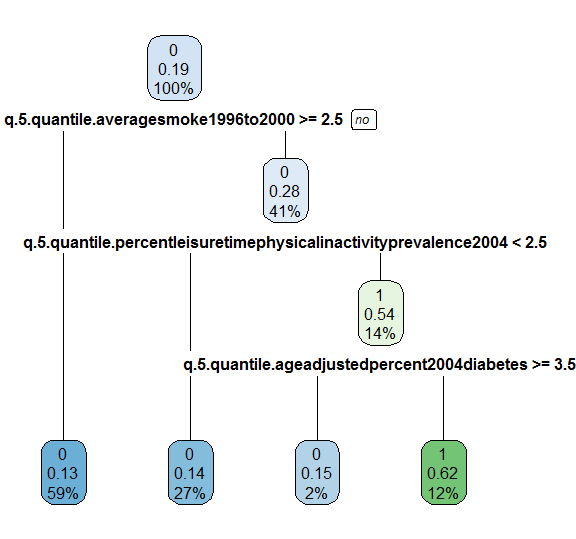
\includegraphics[width=3.25in]{decision-tree-01-paraclique-no-clustering.png}
\caption{Decision tree based on paraclique features, no clustering}
\label{decision.tree.01}
\end{figure}

\begin{figure}[!t]
\centering
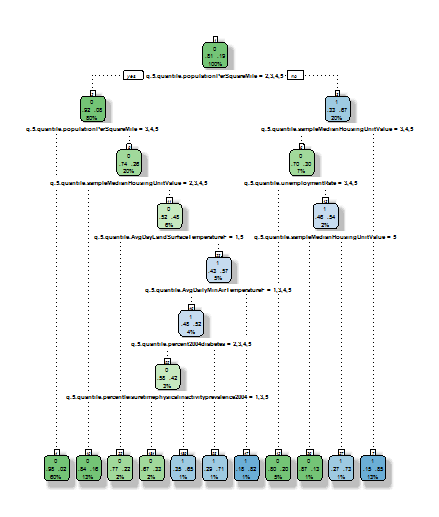
\includegraphics[width=3.25in]{decision-tree-02-all-no-clustering.png}
\caption{Decision tree based on statistical features, no clustering}
\label{decision.tree.02}
\end{figure}

\begin{figure}[!t]
\centering
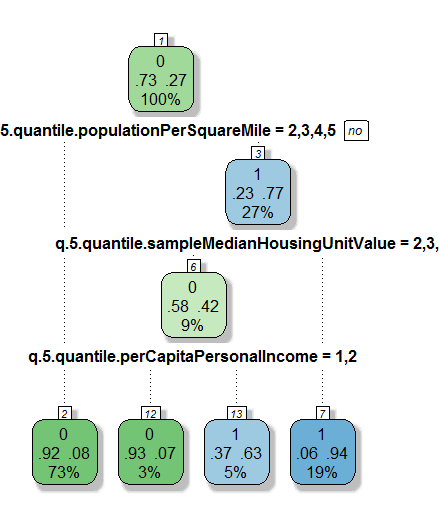
\includegraphics[width=3.25in]{decision-tree-02-cluster-1.png}
\caption{Decision tree based on statistical features, no clustering}
\label{decision.tree.02.1}
\end{figure}

\begin{figure}[!t]
\centering
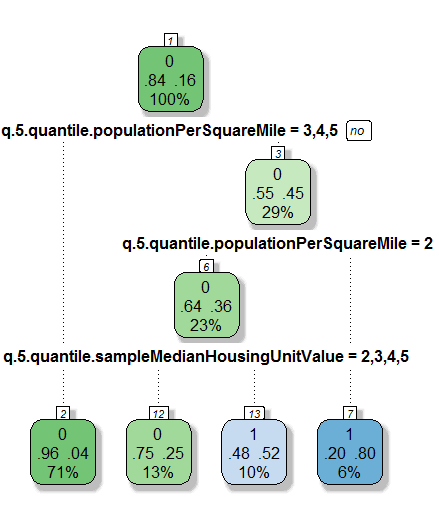
\includegraphics[width=3.25in]{decision-tree-02-cluster-2.png}
\caption{Decision tree based on statistical features, no clustering}
\label{decision.tree.02.2}
\end{figure}

\begin{figure}[!t]
\centering
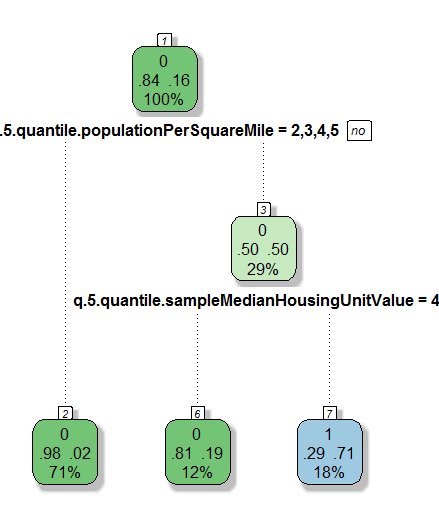
\includegraphics[width=3.25in]{decision-tree-02-cluster-3.png}
\caption{Decision tree based on statistical features, no clustering}
\label{decision.tree.02.3}
\end{figure}

%%%%%%%%%%%%%%%%%%%%%%%%%%%%%%%%%%%%%%%%%%%%%%%%%%%%%%%%%%%%%%%%%%%%%%%%%%%%%%%%
% Tables

\begin{table}[!t]
\renewcommand{\arraystretch}{1.3}
\caption{Confusion Matrix for Tree 1}
\label{table.confusion.matrix.01}
\centering
\begin{tabular}{ccc}
\hline
 & True &  \\
Predicted & 0 & 1 \\
0 & 459 & 97 \\
1 & 11 & 34 \\
\hline
\end{tabular}
\end{table}

\begin{table}[!t]
\renewcommand{\arraystretch}{1.3}
\caption{Confusion Matrix for Tree 2}
\label{table.confusion.matrix.02}
\centering
\begin{tabular}{ccc}
\hline
 & True &  \\
Predicted & 0 & 1 \\
0 & 445 & 45 \\
1 & 25 & 86 \\
\hline
\end{tabular}
\end{table}

\begin{table}[!t]
\renewcommand{\arraystretch}{1.3}
\caption{Accuracy from Feature Reduction Methods on Data Set 1}
\label{table.feature.reduction.accuracy.01}
\centering
\begin{tabular}{ccc}
\hline
Method & Unpruned Accuracy & Pruned Accuracy \\
\hline 
${\chi}^2$ & 0.8040 & 0.7995 \\
Symmetrical Uncertainty & 0.8317 & 0.8316 \\
Gain Ratio & 0.8317 & 0.8316 \\
\hline
\end{tabular}
\end{table}

\begin{table}[!t]
\renewcommand{\arraystretch}{1.3}
\caption{Accuracy from Feature Reduction Methods on Data Set 2}
\label{table.feature.reduction.accuracy.02}
\centering
\begin{tabular}{ccc}
\hline
Method & Unpruned Accuracy & Pruned Accuracy \\
\hline 
${\chi}^2$ & 0.8892 & 0.8893 \\
Symmetrical Uncertainty & 0.8887 & 0.8888 \\
Gain Ratio & 0.8887 & 0.8888 \\
\hline
\end{tabular}
\end{table}

\begin{table}[!t]
\renewcommand{\arraystretch}{1.3}
\caption{Accuracy of Trees from K-means Clusters on Data Set 1}
\label{table.kmeans.accuracy.01}
\centering
\begin{tabular}{ccc}
\hline
Cluster \# & Unpruned Accuracy & Pruned Accuracy \\
\hline 
1 & 0.8190 & 0.8189 \\
2 & 0.8438 & 0.8441 \\
3 & 0.8456 & 0.8407 \\
\hline
\end{tabular}
\end{table}

\begin{table}[!t]
\renewcommand{\arraystretch}{1.3}
\caption{Accuracy of Trees from K-means Clusters on Data Set 2}
\label{table.kmeans.accuracy.02}
\centering
\begin{tabular}{ccc}
\hline
Cluster \# & Unpruned Accuracy & Pruned Accuracy \\
\hline 
1 & 0.8669 & 0.8690 \\
2 & 0.7983 & 0.7919 \\
3 & 0.9919 & 0.9919 \\
\hline
\end{tabular}
\end{table}

%%%%%%%%%%%%%%%%%%%%%%%%%%%%%%%%%%%%%%%%%%%%%%%%%%%%%%%%%%%%%%%%%%%%%%%%%%%%%%%%
% References

% can use a bibliography generated by BibTeX as a .bbl file
% BibTeX documentation can be easily obtained at:
% http://mirror.ctan.org/biblio/bibtex/contrib/doc/
% The IEEEtran BibTeX style support page is at:
% http://www.michaelshell.org/tex/ieeetran/bibtex/
%\bibliographystyle{IEEEtran}
% argument is your BibTeX string definitions and bibliography database(s)
%\bibliography{IEEEabrv,../bib/paper}
%
% <OR> manually copy in the resultant .bbl file
% set second argument of \begin to the number of references
% (used to reserve space for the reference number labels box)

% JSS steps to compile latex + biblatex
% 1. pdflatex traffic-classification.tex
% 2. bibtex traffic-classification (will look for .aux extension, do not specify in argument though)
% 3. pdflatex traffic-classification.tex
% 4. pdflatex traffic-classification.tex (again)

\bibliographystyle{ieeetr}
\bibliography{datta,kershenbaum,juarez,fselector,hartigan,bramer,aggarwal,quinlan,quinlan2,rpart,raman}

\end{document}
